\documentclass[11pt]{article}
\usepackage{acl-ijcnlp2009}
\usepackage{times}
\usepackage{url}
\usepackage{latexsym}
\usepackage{amsmath, amsthm, amssymb, algorithm, algorithmic}
%\setlength\titlebox{6.5cm}    % You can expand the title box if you
% really have to

\newcommand{\mnote}[1]{\marginpar{
    \vskip-\baselineskip \raggedright\footnotesize
    \itshape\hrule\smallskip\tiny{#1}\par\smallskip\hrule}}

%\newcommand{\mnote}[1]{}

\title{Identifying Relational Knowledge for Textual Entailment}

\author{}

\date{}

\begin{document}

\maketitle

\begin{abstract}
We present a novel approach to identifying relations between a pair of
concepts. We focus on identifying relations that are essential to
support textual inference: determining whether two concepts have an
ancestor relation, a sibling relation, or no relation. We develop a
machine learning-based approach that makes use of Wikipedia as a main
source for background knowledge, but we also propose an effective
approach of searching the Web to improve the coverage of our method
and support inference between concepts not present in Wikipedia. Our
key innovation is that, in order to accurately determine the relations
between concepts $C_1$ and $C_2$, we consider an automatically
generated collection of related concepts, evaluate all pairwise
relations, and use constraint-based inference to force them to cohere,
thus improving the local prediction of the pairwise relation
identification. We demonstrate that the inference technique
significantly enhances the local prediction methods and consequently
exhibit very large improvements over methods using existing knowledge
sources.

%%% Local Variables: 
%%% mode: latex
%%% TeX-master: "jupiter"
%%% End: 

\end{abstract}

\section{Introduction}
\label{sec:intro}
\newcommand{\ignore}[1]{}

%The Introduction should contain the followings.
%1. A meaningful example extracted from RTE data sets. This example demonstrates the need of relation detection applied directly to textual inference.
%2. Open and traditional relation extraction and their limitation in natural language inference.
%3. Natural logic for textual inference.
%4. Our system.
%5. Table of content of the paper.
Inference in natural language requires the use of large amounts
of background knowledge. For example, it may be important to
know that a {\em blue Toyota} is not a {\em red Toyota} nor a
{\em blue Honda} but that all are cars, and even Japanese made
cars. This is a different problem than variations of relation
extraction studied in the literature that aim at extracting
relations between entities that co-occur in a given snippet of
text. While the extraction of knowledge of this sort has also
been discussed in the literature, it has been studied mostly in
the context of large scale knowledge acquisition - extract all
{\em easy to find} facts in a given
corpus~\cite{banko-etzioni:2008:ACLMain,davidov-rappoport:2008:ACLMain2,pacsca-vandurme:2008:ACLMain,bunescu-mooney:2007:ACLMain}.
This knowledge is typically existential; e.g., while it is true
that A is of type B, say, it is not clear if it is commonly B;
moreover, if the textual inference system needs to know if A
and B are related, and how, this relation will appear in the
acquired knowledge base only if A and B have occurred in close
proximity in a sentence (and in a easy to understand way).
Consequently, it is difficult for a textual inference system to
benefit from the knowledge acquired this way. Indeed, we know
of no successful application of the large scale existential
knowledge acquisition efforts to textual inference.

In the context of Textual Entailment, for
example~\cite{DaganGlMa06,HaghighiNMa05,BGPRS05}, it has been
argued, e.g., \cite{maccartney-manning:2008:PAPERS}) that many
inferences are largely compositional and depend on the ability
to recognize specific  relations between entities, noun
phrases, verbs, adjectives etc. For example, it is often
necessary to know of an {\em ancestor} relation (and its
directionality) in order to deduce that a statement with
respect to the {\em child} (e.g., George Bush) holds for an {\em ancestor}
(e.g., a republican leader). This is illustrated in the
following example, taken from the RTE4 test suite:

{\small
\begin{quote}

{\bf T}: Nigeria's National Drug Law Enforcement Agency (NDLEA)
has seized 80 metric tonnes of cannabis in one of its largest
ever hauls, officials say.

{\bf H}: Nigeria seizes 80 tonnes of drugs.
\end{quote}
}

Similarly, it is often important to know of a {\em cousin}
relation to infer that a statement about Sun may {\em
contradict} an identical statement with respect to HP (at least
without additional information) since these are {\em different}
companies. This is illustrated in the following example (where
inference requires both identifying a cousin and an
ancestor relation):

{\small
\begin{quote}

{\bf T}: A strong earthquake struck off the southern tip of
Taiwan at 12:26 UTC, triggering a warning from Japan's
Meteorological Agency that a 3.3 foot tsunami could be heading
towards Basco, in the Philippines.

{\bf H}: An earthquake strikes Japan.
\end{quote}
}

This paper proposes to address the problem of relation
identification and classification in a form that is directly
applicable to textual inference.
%
Specifically, our system accepts two input arguments (entities
or noun phrases) and detects the relation between them along
with its possible label (e.g. {\em economic problems} is a
possible class for {\em global warming} and {\em food crisis}).
We focus here on the {\em ancestor} relation and the {\em
cousin} relation, that were identified as key relations also
in \cite{maccartney-manning:2008:PAPERS} (the {\em cousin}
relation is call an {\em alternation} there, and the {\em ancestor} relation is call {\em forward entailment} and {\em backward entailment}). Following the
inference logic developed there, we expect that the resource we
develop in this work can be used compositionally  to support
robust textual inference.

\ignore{ Our approach can discover whether two input entities
pose an alternation (or non-exhautive exclusion) relation ({\em
red} $|$ {\em green}), forward entailment ({\em Mel Gibson}
$\sqsubset$ {\em actor}), reverse entailment ({\em flower}
$\sqsupset$ {\em lily}), or independence ({\em Boeing 747} $\#$
{\em Valentine}). }

We develop an approach that makes use of Wikipedia to recognize
the classify the relations between a pair of arguments on the
fly. While Wikipedia is vast resource that is rapidly being
updated, our approach needs to take into account that it is
developed by a large number of people, and is thus very noisy
and non-uniform. Our algorithmic approach therefore treats
Wikipedia and its category structure as an open resource and
uses statistical text mining techniques to get robust
information from this noisy resource.

For example, the entity {\em Ford} appears many times in
Wikipedia, and is part of a large number of categories. We need
to disambiguate it and determine which category it belongs to
and, within this category, which specific entity is intended.
%For disambiguation, we make use of the context provided by the
%pair - Ford in (Ford, Nixon) is probably different than the one
%in (Ford, Chevrolet)  and possibly even in (Ford, Iacocca).
We
%also
make use of a notion of prominence with respect to a given
text collection (in this case, with respect to Wikipedia
itself) under the assumption that in textual entailment
applications we are in search of some notion of "common sense"
knowledge.

We evaluate our system by comparing its performance over a
large number of pairs chosen from over 40 classes, with a large
scale effort done in forming the extended WordNet \cite{Snow2006}. We show significantly better results in
terms of coverage and accuracy.
Furthermore, we show that even when all entities are covered by the extended WordNet, our system still significantly outperforms the baseline.
%We also show examples for the
%contribution our approach can make in the context of textual
%entailment.

The rest of this paper is organized as follows. In Section
\ref{sec:relatedwork}, we briefly mention about previous work that inspires the proposal of our approach.
Section \ref{sec:approach} formalizes the problem and describes our
algorithmic approach to relation detection and classification.
Our experiments and results are described in Section
\ref{sec:experiments}. Discussion and future work are in
Section \ref{sec:discussion}. We
give the concluding remarks of our paper in Section \ref{sec:conclusion}.

%
%%The Introduction should contain the followings.
%%1. A meaningful example extracted from RTE data sets. This example demonstrates the need of relation detection applied directly to textual inference.
%%2. Open and traditional relation extraction and their limitation in natural language inference.
%%3. Natural logic for textual inference.
%%4. Our system.
%%5. Table of content of the paper.

%Many natural language processing applications require semantic inference which, in turn, demands a common framework for applied semantics. Recently, textual entailment has shown considerable promise as a framework to apply textual inference \cite{Dagan05thepascal}.

%Among several approaches developed to achieve the ultimate goal of the textual entailment task, the approach based on a model of natural logic, which utilizes lexical entailment relations to do inference, has proved to be very promising \cite{maccartney-manning:2008:PAPERS}.

%However, this approach requires an effective way to exploit the background knowledge that provides useful and accurate information to the inference process.  Most of the current approaches in relation extraction look at collections of text and extract all possible facts from these corpora \cite{banko-etzioni:2008:ACLMain,davidov-rappoport:2008:ACLMain2,pacsca-vandurme:2008:ACLMain,bunescu-mooney:2007:ACLMain}. However, it is difficult for a textual inference system to get benefit from this direction because of two difficulties: (1) the extracted knowledge may not be particularly well-suited for natural language inference and (2) knowledge about specific entities in focus may not be associated with the extracted facts due to the inherent characteristics of natural language.

%Consider the following example, drawn from the RTE4 test suite (pair id=``74'').

%\begin{quote}

%{\bf T}: With tales of rising seas and talk of human solidarity, world leaders at the first United Nations climate summit sought Monday to put new urgency into global talks to reduce {\em global warming} emissions.

%{\bf H}: UN summit targets global {\em food crisis}.

%\end{quote}

%This example, in the 2-way classification textual entailment task, is tagged as {\bf NO} entailment. One way to induce the answer for this example is that by looking at the pair of entities ({\em global warming}, {\em food crisis}), one can see that the entities are about two {\em economic problems}; and they share the alternation (or non-exhaustive exclusion) relation, which is obvious for human. This, therefore, ensures that {\bf T} and {\bf H} are talking about two different things so that {\bf T} cannot entail {\bf H}. 
%\mnote{[QD:] This paragraph seems to be not clear enough. Revise needed.}
%Nevertheless, it is difficult for an inference system itself to conclude that there are no relation between these two entities to induce a correct answer.

%In this paper, we propose a novel approach that uses Wikipedia as the background knowledge to detect the relations between entities in real-time. We position the problem of relation detection in the context of the textual entailment task, where relations between entities are used to do textual inference. Our system accepts two input entities and detect the relation between them along with their possible classes (e.g. {\em economic problems} is a possible class for {\em global warming} and {\em food crisis}).
%\mnote{[QD:] I don't like the way I express my idea here. The words that I am using are not interesting, professional, and convincing. I have not known how to make it better so far.}
%Our approach can discover whether two input entities pose an alternation (or non-exhautive exclusion) relation ({\em red} $|$ {\em green}), forward entailment ({\em Mel Gibson} $\sqsubset$ {\em actor}), reverse entailment ({\em flower} $\sqsupset$ {\em lily}), or independence ({\em Boeing 747} $\#$ {\em Valentine}).
%The experiments on the data of 40 classes of instances \cite{citeulike:1587018} show that our best system in relation detection achieve over 80\% of accuracy, which outperforms the baseline at more than 40\%.

%Furthermore, we evaluate our system on the examples extracted from all RTE data sets and FraCaS test suite \cite{Cooper1996FraCaS}. The experiments also show that our system is very valuable for textual inference.

%The rest of this paper is organized as follows. In Section \ref{sec:relationdetection}, we introduce the problem of relation detection and its role in natural logic inference. Section \ref{sec:approach} formalizes the problem and proposes our approach to relation detection. Our experiments and results are described in Section \ref{sec:experiments}. Discussion and related work are in Section \ref{sec:discussion}, and \ref{sec:relatedwork}. We give the concluding remarks of our paper and suggest future work in Section \ref{sec:conclusion}.


\section{Previous Work}
\label{sec:relatedwork}
To the best of our knowledge, no previous study has directly addressed
the problem of identifying taxonomic relation between two given
concepts. However, there are several work which acquires structured
taxonomies and ontologies.

\ignore{Several lines of work share similarities to the work presented
  here. One line of work makes use of the web and exploits the fact
  that many relations are expressed explicitly and locally, typically
  within a single sentence. It uses this to discover terms which have
  hypernyms or coordinate relations \cite{citeulike:282193,Snow2006}
  or to expand or refine members in a semantic class (given seeds or
  the semantic class itself)
  \cite{WangCohen09,VyasPantel09,kozareva-riloff-hovy:2008:ACLMain,4470258,banko-etzioni:2008:ACLMain}.
  A second line of work attempts to classify pre-specified relations
  \cite{citeulike:454000,Sekine06,RothYi04} and typically makes use of
  supervised or semi-supervised learning techniques.

  The later line of work is different from ours in terms of goals and
  techniques. It considers relations such as ``SpouseOf" of ``BornIn"
  and relies on the relation being expressed in close proximity,
  typically within a sentence, and on training supervised classifiers.
  The line of work which makes use of the web is similar to ours in
  terms of the final task, but is different in its assumptions and
  techniques---it mostly relies on the fact that due to redundancy of
  information in the web, and presumes that many related terms will appear often
  enough in some simple explicit form in close proximity.}

In \cite{ilprints665} and \cite{Snow2006}, the authors constructed
classifiers to identify hypernym relationship between concepts. The
classifiers is then used to augment WordNet \cite{Fellbaum98} with
over $400,000$ synsets. 

\ignore{ They combine their hypernym-only classifier and the
  ($m$,$n$)-cousin classifier with the evidence features to recognize
  the hypernym and cousin relationships among nouns.  Their inferred
  taxonomy achieves the best performance after adding 30,000 novel
  hyponyms compared to those in WordNet-2.1.  They show that their
  system relatively improves F-score by 23\% over the WordNet-2.1
  hypernym classifier.}

\ignore{ Using similar techniques to the aforementioned line of work,
  there has been a large body of work on automatically expanding a set
  of entities given some seeds that belong to a semantic class or the
  class itself. A typical application of this research is that of
  expanding, correcting or refining Google
  Sets\footnote{http://labs.google.com/sets}.

%
  % The common input of systems in this direction is a set of seeds in
  % a particular semantic class that one wishes to get other members
  % of that class.
%
  Typically, these methods search the web for patterns around the
  seeds and bootstrap to other semantically similar members of the
  class~\cite{kozareva-riloff-hovy:2008:ACLMain,talukdar-EtAl:2006:CoNLL-X}.
  Alternatively, \cite{4781230,4470258} use the surrounding contexts
  of the seeds in semi-structured text to extract other members of the
  set. Similarly,
  \cite{citeulike:1587018,pacsca-vandurme:2008:ACLMain} automatically
  acquire open-domain classes of entities and attributes by using
  very little supervised seed information.
  % Web documents and query logs are used in the acquisition process.
}

\ignore{The key difference between this line of work and the approach
  we develop here is that we are given two concepts and must determine
  the relation between them. The coverage of the aforementioned
  methods is lacking since they rely on concepts appearing in close
  proximity with specific patterns that reveal their relation. It is
  likely, however, that our input concepts never occur together in a
  given sentence even though they are clearly related. As we
  show, we can robustly and accurately determine these relations,
  significantly outperforming state of the art acquisition methods
  such as \cite{Snow2006}.}

\cite{wikitaxo07} generated a taxonomy using Wikipedia as the
knowledge source. They used the Wikipedia category system as a
conceptual network consisting of subsumption ({\em isa})
relations. \cite{suchanek2007WWW} presented the the \textsc{Yago}
ontology, which was automatically constructed using both Wikipedia and
WordNet. The \textsc{Yago} approach built on the {\em infoboxes} and
{\em category pages} in Wikipedia and linked to a clean taxonomy of
concepts in WordNet. \textsc{Yago} provides many useful relations such
as {\em subClassOf}, {\em bornOnDate}, and {\em type}.  Our work
differs from this line of work because we do not build a knowledge
base, but rather directly identify taxonomic relations between two
given concepts.

% % Story of previous work

% % 1. Summarize the work on discovering terms which have hypernym or
% % coordinate relation. E.g. the work of Marti Hearst 1992, Rion Snow
% % 2006, Hovy 2005.

% % 2. Summarize the work about expanding sets and refining set
% % expansion. E.g. the work of Cohen 2007, 2008, 2009, Hovy 2007, Pasca
% % 2007, 2008, Sarmento 2007, Pantel 2009

% % 3. Perhaps also summarize the work of relation classifiercaiton. E.g. Zhu Zhang 2004, 

% % 4. Claim that other work using supervised learning with pre-defined
% % list of relation and domain dependency, we do different things: (a)
% % supervised learning with arbitrary types of ancestor and cousin
% % relations, (b) we are domain-independent: train on some domains and
% % work well in other domains. This is also the contributions of this
% % paper.

% The task of relational knowledge identification can be seen as related
% to the work on discovering terms which have hypernym or coordinate
% relation \cite{citeulike:282193,Snow2006}, expanding or refining sets
% of a semantic class from a list of given seeds or the semantic class
% itself
% \cite{WangCohen09,VyasPantel09,kozareva-riloff-hovy:2008:ACLMain,4470258},
% or classifying pre-specified relations \cite{citeulike:454000}.

% In \cite{ilprints665}, the authors construct a hypernym-only
% classifier using the dependency path patterns discovered in the
% sentences that contain noun pairs in hypernym and hyponym
% relations. Furthermore, they show that using coordinate terms can help
% improve the recall of the hypernym classifier. The best system in
% their work is a hypernym-only classifier additionally trained with
% hundred thousands of dependency paths extracted from the Wikipedia corpus.
% The system outperforms the best WordNet classifier in identifying
% coordinated terms by relatively improving F-score by over
% 54\%. Recently, \cite{Snow2006} propose a method to train their
% ($m$,$n$)-cousin relationship classifier. They combine their
% hypernym-only classifier and the ($m$,$n$)-cousin classifier with the
% evidence features to recognize the hypernym and cousin relationships
% among nouns. Their inferred taxonomy achieves the best performance
% after adding 30,000 novel hyponyms compared to those in
% WordNet-2.1. They show that their system relatively improves F-score
% by 23\% over the WordNet-2.1 hypernym classifier.

% There has been a large body of work on automatically expand a set of
% entities given some seeds of a semantic class or the class itself. A
% typical application of this research is Google
% Sets\footnote{http://labs.google.com/sets}. The common input of
% systems in this direction is a set of seeds in a particular semantic
% class that one wishes to get other members of that class.  The common
% approach is to do bootstrapping on the input seeds to get the patterns
% around the seeds in unstructured text by searching the Web, then
% extract other semantically similar members of the class, and vice
% versa
% \cite{kozareva-riloff-hovy:2008:ACLMain,talukdar-EtAl:2006:CoNLL-X}. On
% the other hand, \cite{4781230,4470258} use surrounding contexts of
% seeds in semi-structured text to extract other members of the set.
% \cite{citeulike:1587018,pacsca-vandurme:2008:ACLMain} proposed
% approaches to automatically acquire open-domain classes of entities
% and attributes by using very little supervised seed information. Web
% documents and query logs are used in the acquisition process. Other
% approaches in information extraction include constructing relation
% classifiers on a pre-defined set of specific relations such as {\em
%   People, Organization, and Location}, or exhaustively searching and
% extracting all possible relations and related concepts
% \cite{citeulike:454000,banko-etzioni:2008:ACLMain}.

% In this paper, we solve the problem of relational knowledge
% identification which is in a different context with other information
% extraction problems. The key difference is that we address the problem
% of identification which answers the question if two input concepts
% hold an relation, whereas an expanding process tries to extract as
% many semantically similar concepts as possible without any specific
% concepts in mind. Although the latter task can produce many good sets
% through the expansion process, there is no guarantee about the
% completeness of the sets. Therefore, they are not useful in
% identifying relations between two given concepts of interest.


%%% Local Variables: 
%%% mode: latex
%%% TeX-master: "jupiter"
%%% End: 


%\section{Relation Detection for Natural Language Inference}
%\label{sec:relationdetection}
%This section should have two sub-sections.

1. Relation Detection is Different to Relation Extraction

2. The Importance of Relation Detection in Natural Language Inference

%\section{Identifying Ancestor and Cousin Relationships}
\section{Relation Identification}
\label{sec:approach}
%This section presents the approach to relation detection using Wikipedia category structure.

%There should be some important sub-sections.

%1. Wikipedia Category Structure

%2. Formalizing the problem of Detecting Relations with Wikipedia Categories

%3. Prominence-base Search: Focusing on Important concepts

%4. Ranking the Class of Entities

%5. Lexical Matching of Categories

%6. Entity Class Disambiguation in Textual Inference

In this section we first give our definitions of ancestor and cousin relationships. After that in section \ref{sec:wikipedia-category-structure}, we describe the Wikipedia category structure. We show that the Wikipedia category structure is naturally fit with the demand of identifying hierarchical relationship between concepts. We then present our algorithms and its extension in sections \ref{sec:algorithms} and \ref{sec:prominence}.

\subsection{Ancestor and Cousin Relationships}
\label{sec:definitions}
We follow the definitions in \cite{Snow2006} to define the hypernym and ($m$, $n$)-cousin relationships between senses in WordNet.
In their paper, a hypernym relationship is denoted by $H_{ij}^{n}$ if a sense $j$ is the $n$-th ancestor of a sense $i$ in the hypernym hiararchy.
The notation is simplified to $H_{ij}$ to denote that sense $j$ is an ancestor of sense $i$ at some level.
On the other hand, the sibling relationship between senses $i$ and $j$ is generalized to ($m$, $n$)-cousin relationship which defines that sense $i$ and sense $j$ have their {\em least common subsummer} (LCS) in within exact $m$ and $n$ links, respectively.

We adopt these definitions to define the ancestor and cousin relationships between entities by using Wikipedia articles and Wikipedia category structure, which we will describe in Section \ref{sec:wikipedia-category-structure}.
We {\em loosely define} that entity $X$ is an ancestor of entity $Y$ if the title of one of the articles about $X$ in Wikipedia {\em matches} one of the categories or ancestor categories of the articles about $Y$ in Wikipedia.
We also follow the ($m$, $n$)-cousinhood definition to define the cousin relationship. Entities $X$ and $Y$ are cousins if the articles about $X$ in Wikipedia {\em share} one or more categories with the articles about $Y$, also in Wikipedia.

For instance, follow our definition, we can verify that {\em color} and {\em red} have an ancestor relationship because there is an article entitled ``Red'' (for entity {\em red}) that belongs to the category {\bf Color} which is the title of another article about entity {\em color}.
We also can verify that {\em red} and {\em green} belong to two articles (one entitled ``Red'', and the other one entitled ``Green'') which share a common caretory {\bf Color}. Therefore, they are cousins.


\subsection{Category Structure of Articles in Wikipedia}
\label{sec:wikipedia-category-structure}
Wikipedia\footnote{http://www.wikipedia.org} is a freely available encyclopedia on the web developed by the contribution of a huge number of internet users around the world. Recently, more and more research that focuses on exploiting the valuable knowledge resources in Wikipedia has been carryied out \cite{CRRS08,richman-schone:2008:ACLMain,suchanek2007WWW,citeulike:2157093}.
There are millions of articles in Wikipedia; and this number is increasing rapidly day by day.
At the time of February, 2009, there are 2,738,772 articles in the English Wikipedia\footnote{http://en.wikipedia.org/wiki/Size\_of\_Wikipedia}.
Each article in this encyclopedia is collaboratively written by volunteers and categorized into different categories by the authors of the article.
One can observe that, although the content of articles in Wikipedia may contain false information at some point in its development, the categories of an article are quite determinable. 

Essentially, as a nature of things, a certain concept may belong to several topics. Similarly, each article in Wikipedia will often be in several categories. And each category itself is also an article in Wikipedia; so it has its own super-categories. For example, the article with the title $t = $ {\em George W. Bush} belongs to a set of categories at the fist level $\mathcal{C}^{1} = $ \{{\em Category:George W. Bush}, {\em Category:Presidents of the United States}, {\em Category:Harvard University alumni}, ...\}; at the second level of $t$ we have
%that $t = $ {\em Category:Presidents of the United States} is in the categories of
$\mathcal{C}^{2} = $ \{{\em Category:Heads of government by country}, {\em Presidents by country}, {\em American politicians}, ...\}.

From the properties of categories, they do not form a strict hierarchy or tree of categories. This allows multiple categorization schemes to co-exist simultaneously. As a guideline in constructing categories of Wikipedia articles, there is no constraints from constructing loops in the category space, but this is strongly discouraged. In our work, we consider the Wikipedia category structure as a directed acyclic graph.

Interestingly, as a matter of fact, articles in the same category or in its sub-categories are considered siblings. This fact is stated clearly in the guideline of the category structure in Wikipedia\footnote{http://en.wikipedia.org/wiki/Wikipedia:Category}. For one who wants to find the siblings of an article, he or she can not only look at the articles in the category but also can find more in its sub-categories. This valuable property of Wikipedia category directly suggests an efficient approach to identify relations between entities as long as they have their own article in Wikipedia.

%\subsection{Identifying Ancestor and Cousin Relationships Using Wikipedia Categories}
\subsection{Identifying Entity Relations Using Wikipedia Categories}
\label{sec:algorithms}

In this section, we present our algorithms for identifying the possible ancestor and cousin relationships between entities.

For any entity $X$, we define the followings variables.

\begin{itemize}
\item $\mathcal{T_{X}}$: the set of the top ranked articles returned by searching $X$ in in the pool of all {\em article titles} in Wikipedia.
\item $\{ c_{t_{X}}^{L} \}$: the set of all categories extracted for the titles $t_{X} \in \mathcal{T_{X}}$ by going up to $L$ levels of ancestor.
\item ${\mathcal C}_{X} = \bigcup_{t_{X} \in {\mathcal T}_{X}} \{{c_{t_{X}}^{L}\}}$: the union set of categories extracted for all titles in $\mathcal{T_{X}}$ by going up to $L$ levels of ancestor.
\end{itemize}

Futthermore, for a category, we can possibly determine its generalized name which we call generalized category, and its domain by analyzing the category using lexical and syntactic information. For instance, with category $c$ = {\em Cities in the United States}, we locate its generalized name as {\em Cities}, and its domain as {\em the United States}. By this, we define the followings variables.

\begin{itemize}
\item ${\mathcal G}_{X}$: the union of all generalized category names of the categories of entity $X$, in ${\mathcal C}_{X}$.
\item ${\mathcal D}_{X}$: the union of all domains of the categories of entity $X$, in ${\mathcal C}_{X}$.
\end{itemize}

\begin{algorithm} [t]
{\small
\caption{AncestorRelationIdentification}
\label{algAncestorIdentifying} 
\begin{algorithmic}[1]
\STATE Input: Wikipedia index $I_{W	}$ 
\STATE $\qquad$$K$: number of top documents 
\STATE $\qquad$$L$: number of levels of ancestor. 
\STATE $\qquad$$(X, Y)$: two input entities. 
\STATE Output: $0$: no ancestor relationship. 
\STATE $\qquad\quad$$1$: $X$ is an ancestor of $Y$.

\STATE ${\mathcal T_{X}}$ $\leftarrow$ SearchByTitle($X$, $I_{W}$, $K$);
\STATE ${\mathcal T_{Y}}$ $\leftarrow$ SearchByTitle($Y$, $I_{W}$, $K$);

\STATE ${\mathcal C}_{Y} = \{\}$;

\FOR{each $t_{Y} \in {\mathcal T}_{Y}$}
\STATE $\{c_{t_{Y}}^{L}\} \leftarrow$ RecursivelyExtractCate$(t_{Y},L)$
\STATE ${\mathcal C}_{Y} = {\mathcal C}_{Y} \cup \{c_{t_{Y}}^{L}\}$;
\ENDFOR

\STATE ${\mathcal G}_{Y} \leftarrow$ CategoryGeneralization$({\mathcal C}_{Y})$;
\STATE ${\mathcal D}_{Y} \leftarrow$ DomainExtraction$({\mathcal C}_{Y})$;

\STATE ${\mathcal E}_{Y} = {\mathcal C}_{Y} \cup {\mathcal G}_{Y} \cup {\mathcal D}_{Y}$

\FOR {each $t \in {\mathcal T_{X}}$}
\IF {(Match $(t,{\mathcal E}_{Y})$)}
\RETURN {1};
\ENDIF
\ENDFOR

\RETURN 0;

\end{algorithmic} 
}
\end{algorithm} 


Algorithm \ref{algAncestorIdentifying} describes our approach to identifying the ancestor relationship between two input entity $X$ and $Y$. The algorithm returns ${\bf 1}$ as an indicator for $X$ to be an ancestor of $Y$. In lines 7 and 8 of the algorithm, we respectively search for articles in Wikipedia that contain all tokens of $X$ and $Y$ in their titles. Only top $K$ most relevant titles are returned. From line 9 to line 13, all categories up to $L$ levels of ancestor of the retrieved articles of $Y$ are collected. We extract the generalized category names and domains of all extracted categories of $Y$ by calling functions {\em CategoryGeneralization} and {\em DomainExtraction}, respectively. After that, from line 16 to 22, the union set ${\mathcal E}_{Y}$ of all categories, their generalized category names, and their domains is produced and compared with the article titles of $X$. If there is any {\em match} happens between titles in ${\mathcal T}_{X}$ and elements in ${\mathcal E}_{Y}$, the algorithm returns the answer indicating that $X$ is an ancestor of $Y$ and terminates, otherwise, the algorithm concludes that there is no ancestor relationship between $X$ and $Y$.

\begin{algorithm} [t]
{\small
\caption{CousinRelationIdentification}
\label{algCousinIdentifying} 
\begin{algorithmic}[1]
\STATE Input: Wikipedia index $I_{W	}$ 
\STATE $\qquad$$K$: number of top documents 
\STATE $\qquad$$L$: number of levels of ancestor. 
\STATE $\qquad$$(X, Y)$: two input entities. 
\STATE Output: $(0,\{\})$: no cousin relationship. 
\STATE $\qquad\quad$$(1,{\mathcal N})$: $X$ and $Y$ are cousin.
\STATE $\quad\qquad$${\mathcal N}$ is the list of possible class names. 

\STATE ${\mathcal T_{X}}$ $\leftarrow$ SearchByTitle($X$, $I_{W}$, $K$);
\STATE ${\mathcal T_{Y}}$ $\leftarrow$ SearchByTitle($Y$, $I_{W}$, $K$);

\STATE ${\mathcal C_{X}}$ $\leftarrow$ CategoryExtraction(${\mathcal T}_{X}$, $L$);
\STATE ${\mathcal C_{Y}}$ $\leftarrow$ CategoryExtraction(${\mathcal T}_{Y}$, $L$);

\STATE ${\mathcal G}_{X} \leftarrow$ CategoryGeneralization$({\mathcal C}_{X})$;
\STATE ${\mathcal G}_{Y} \leftarrow$ CategoryGeneralization$({\mathcal C}_{Y})$;

\STATE ${\mathcal N} = \text{Match}({\mathcal C}_{X}, {\mathcal C}_{Y}) \cup \text{Match}({\mathcal G}_{X}, {\mathcal G}_{Y})$

\IF {(${\mathcal N} \neq \emptyset$)}
\RETURN (1, ${\mathcal N}$);
\ELSE
\RETURN (0, $\{\}$);
\ENDIF

\end{algorithmic} 
}
\end{algorithm} 

The cousin relation identifier is described in Algorithm \ref{algCousinIdentifying}. In lines 8 and 9, the articles in Wikipedia which have the titles containing all words in two entities are retrieved, respectively. After that, the union set of categories are extracted by going upto $L$ levels of ancestor, for all titles in $\mathcal{T_{X}}$, line 10, and $\mathcal{T_{Y}}$, line 11. Function {\em CategoryExtraction} has been actually showed in Algorithm \ref{algAncestorIdentifying} from line 9 to 13. After that, the generalized category names of all extracted categories are induced for $X$ and $Y$. Finally, the matching functions will look for matches between two sets of categories and generalized category names. If there is any match happening, it will be put into a list of all possible class names for $X$ and $Y$. The algorithm is going to return the class name list along with an indicator indicating that $X$ and $Y$ have cousin relationship. Otherwise, it returns {\bf 0} for no relation between $X$ and $Y$.

\begin{algorithm}[t]
{\small
\caption{RelationIdentification}
\label{algRelationIdentifying} 
\begin{algorithmic}[1]
\STATE Input: Wikipedia index $I_{W	}$ 
\STATE $\qquad$$K$: number of top documents 
\STATE $\qquad$$L$: number of levels of ancestor. 
\STATE $\qquad$$(X, Y)$: two input entities. 
\STATE Output: $(0, \{\})$: $X$ and $Y$ have no relationship. 
\STATE $\qquad$$(1, \{\})$: $X$ is an ancestor of $Y$,
\STATE $\qquad$$(2, \{\})$: $Y$ is an ancestor of $X$,
\STATE $\qquad$$(3, {\mathcal N})$: $X$ and $Y$ are cousin,
\STATE $\quad\qquad$${\mathcal N}$ is the list of possible class names. 

\IF {(AncestorRelationIdentification($X$,$Y$))}
\RETURN (1, $\{\}$);
\ELSE
\IF {(AncestorRelationIdentification($Y$, $X$))}
\RETURN  (2, $\{\}$);
\ENDIF
\ENDIF

\STATE $(I, {\mathcal N})$ = CousinRelationIdentification($X$,$Y$)

\IF {($I == 1$)}
\RETURN (3, ${\mathcal N}$);
\ELSE
\RETURN (0, $\{\}$);
\ENDIF

\end{algorithmic} 
}
\end{algorithm} 


After having algorithms to identify ancestor and cousin relations between entities, we design the relation identification algorithm, which is described in Algorithm \ref{algRelationIdentifying}. Input of the algorithm is a pair of entities ($X$, $Y$). The algorithm outputs the predict relationships between $X$ and $Y$, including ancestor, cousin, or no relation. If two entities bind a cousin relationship, the algorithm also returns a list of possible class names of the two entities. For instance, the list of class names would be \{{\em American film actors}, {\em film directors}, ...\} for the input pair ({\em Mel Gibson}, {\em Tom Cruise}). From line 10 to 16, the algorithm first checks if there is ancestor relationship between two entities using Algorithm \ref{algAncestorIdentifying}. The algorithm immediately returns the answer if there is indeed an ancestor relationship between $X$ and $Y$, otherwise, the algorithm continues identifying the possible cousin relationship between two entities. 
Otherwise, the algorithm conclude that there is no relation for two input entities.

% 
%We also define ${\bf I}(\cdot, \cdot)$ as the indicator function that lexically compares two strings and determines whether the two strings are {\em similar}, which will be defined in specific contexts.

%\begin{equation}
%  {\bf I}(u,v) = \begin{cases}
%    1 & \mbox{if $u$ and $v$ are similar} \\
%    0 & \mbox{otherwise}
%    \end{cases}
%    \label{eq:thetaDefinition}
%\end{equation}

%The string arguments of function $f$ can be entities, article titles, categories, generalized names of categories, or domains of categories.

%An entity $X$ is considered a parent of an entity $Y$ if ${\bf I}(X,Y) = 0$ and one of the following conditions is satisfied.

%\begin{itemize}
%\item ${\bf I}(X, c_{Y}) = 1$, where $c_{Y} \in \mathcal{C}_{Y}^{*}$
%\item ${\bf I}(X, g_{Y}) = 1$, where $g_{Y} \in \mathcal{G}_{Y}^{*}$
%\item ${\bf I}(X, d_{Y}) = 1$, where $g_{Y} \in \mathcal{D}_{Y}^{*}$
%\end{itemize}

%Similarly, an entity $X$ is considered a child of an entity $Y$ if ${\bf I}(X,Y) = 0$ and one of the following conditions is satisfied.

%\begin{itemize}
%\item ${\bf I}(c_{X}, Y) = 1$, where $c_{X} \in \mathcal{C}_{X}^{*}$
%\item ${\bf I}(g_{X}, Y) = 1$, where $g_{Y} \in \mathcal{G}_{X}^{*}$
%\item ${\bf I}(d_{X}, Y) = 1$, where $g_{Y} \in \mathcal{D}_{X}^{*}$
%\end{itemize}

%Furthermore, two entities $X$ and $Y$ are considered siblings if ${\bf I}(X,Y) = 0$ and one of the following conditions is satisfied.

%\begin{itemize}
%\item ${\bf I}(c_{X}, c_{Y}) = 1$, where $c_{X} \in \mathcal{C}_{X}^{*}$, and $c_{Y} \in \mathcal{C}_{Y}^{*}$
%\item ${\bf I}(g_{X}, g_{Y}) = 1$, where $g_{X} \in \mathcal{G}_{X}^{*}$, and $g_{Y} \in \mathcal{G}_{Y}^{*}$
%\end{itemize}

%If two entities are determined siblings, their class will be defined by the matched category or matched generalized name.

%\mnote{[QD:] I think this issue can be solved by using WordNet to look up the level of abstraction of the class. In WordNet, the closer a noun to the root node {\bf entity}, the more abstract it is.}

%There is a potential issue with the determined class of two sibling entities. The class can be very abstract, or very specific. Generally, one does not want two entities to be siblings in a very abstract class. XXXXXXXXXXXXXXXXXXXXXXXXXXX to be continue!!!

\subsection{Prominence-based Search}
\label{sec:prominence}
As far as we observe the algorithms, we can see that the {\em SearchByTitle} function guide the identification prediction heavily. If the function returns irrelevant or unimportant articles about entities, we easily get wrong relations. Therefore, designing a good entity search function is important. In this section, we propose an approach called prominence-based search to improve the search results of input entities. Although our initial approach for prominence-based search is simple, it can serve as an disambiguation tool for entities.

We guide the search engine based on an assumption that, without special purpose, people often want to see information known or important entities retrieved when they search for information. We translate this assumption into our search engine by returning only top relevant articles about prominent entities. We measure the prominence of entities by their occurrence in a large text collection. For instance, if one wants to search for entity {\em bush}, the search engine may retrieve thousands of articles including {\em Kate Bush}, {\em William Bush}, {\em Laura Bush}, {\em George W. Bush}, {\em Bush family}, and so on. Among these articles, our system retrieves the ones about {\em George W. Bush}, {\em George H. W. Bush} in the top of the returned article set because their frequency of occurrence dominates other entities.
%Algorithm \ref{alg:prominence-search} present our approach to prominence-based search.

%\begin{algorithm}[t]
%\caption{Prominence-based Search}
%\label{alg:prominence-search} 
%\begin{algorithmic}[1]
%\STATE Input: an entity $X$. 
%\STATE $\qquad$$K$: number of top ranked articles. 
%\STATE $\qquad$${\mathcal D}$: a document collection
%\STATE Output: A ranked list of articles about $X$ based on prominency. 

%\STATE ${\mathcal T}_{X} \leftarrow $ NormalSearchByTitle($X$);
%\STATE ${\mathcal T}$ = \{\};

%\FOR {each $t \in {\mathcal T}_{X}$}
%\STATE $hit = \text{HitCount}(t, {\mathcal D})$;
%\STATE ${\mathcal T} \leftarrow \left< t, hit \right>$;
%\ENDFOR

%\STATE ${\mathcal T} \leftarrow \text{SortByProminence}({\mathcal T})$;

%\RETURN Top $K$ articles from ${\mathcal T}$;

%\end{algorithmic} 
%\end{algorithm} 


%\subsection{The Association of a Title and its Category}

%\subsection{The Issue of Redirect Articles}

%\subsection{Lexical Similarity Matching}



\section{Experiments and Results}
\label{sec:experiments}
In this section, we first describe the datasets. Follow that, we
present the experiments to evaluate our overall system and compare it
with other systems using existing large-scale resources. We also give
a deeper understanding about our system by performing several
experimental analyses.

\subsection{Datasets}
\label{sec:dataset}

In our experiments, two main datasets are used. The first dataset is
generated from 40 semantic classes of almost 11,000 instances. The
original semantic classes were manually constructed\footnote{Private
  communication.}  and was used to evaluate information extraction
tasks as in \cite{citeulike:1587018,pacsca-vandurme:2008:ACLMain}. The
second dataset is generated from 44 semantic classes of more than
10,000 instances used in
\cite{vyas-pantel:2009:NAACLHLT09}\footnote{There were 50 semantic
  classes in the original dataset. We grouped some semantically
  similar classes for the purpose of identifying taxonomic
  relations.}. The original classes of the second dataset were
extracted from Wikipedia lists. In both datasets, we have both types
of closed word semantic class (e.g. {\em chemical element}, {\em
  country}) and open word semantic class (e.g. {\em basic food}, {\em
  hurricane}). Moreover, there are classes with proper nouns
(e.g. {\em actor} with {\em Mel Gibson}) and classes with common nouns
(e.g. {\em basic food} with {\em rice}, {\em milk}).

Several semantic class names in the original data are written in a
short form (e.g. {\em chemicalelem}, {\em proglanguage}). We,
therefore, expand each semantic class name in the original dataset to
some meaningful names which are used by all systems in our
experiments. For example, {\em terroristgroup} is expanded to {{\em
    terrorist group}, {\em torrorism}}.

\begin{table}[!t]
  \small
  \centering
  \begin{tabular}{r|l|l}
    %\hline
    %\multicolumn{3}{|c|}{Concept pair examples} \\
    %\hline
    Relation          & Concept $X$ & Concept $Y$    \\
    \hline
    %\hline
    $X \leftarrow Y$        & actor             & Mel Gibson           \\
    & food              & rice                 \\
    % & wine              & Champagne            \\
    \hline                               
    $X \rightarrow Y$       & Makalu            & mountain             \\
    & Monopoly          & game                 \\
    % & krooni            & currency             \\
    \hline                               
    $X \leftrightarrow Y$   & Paris             & London               \\
    & copper            & oxygen                \\
    % & Nile              & Volga                 \\
    \hline                               
    $X \nleftrightarrow Y$ & Roja              & C++                  \\
    & egg               & Vega                  \\
    % & HotBot            & autism                \\
    %\hline
  \end{tabular}
  \caption{Some examples in our data set.}
  \label{table:examples}
\end{table}


We refer to both name of a semantic classes and its instances as
concepts. An example in the problem of taxonomic relation
identification is a pair of two concepts ($X$, $Y$) such as ({\em
  city}, {\em Dubai}), ({\em lead}, {\em aluminum}). We pair the
semantic classes and instances in the original data set to create
training and testing examples. For each original dataset, we randomly
generate disjoint training and test sets of $12,000$ and $8,000$
examples, respectively. We call the test set from the first and the
second datasets {\bf Test-I} and {\bf Test-II},
respecitively. \ignore{Because {\bf Test-II} contains only {\em
    Wikipedia concepts}, we do not evaluate it the experiments that
  find replacements for {\em non-Wikipedia concepts}.} Table
\ref{table:examples} shows some generated examples. All types of
taxonomic relations including $X \leftarrow Y$, $X \rightarrow Y$, $X
\leftrightarrow Y$, and $X \nleftrightarrow Y$ are covered with a
balanced number of examples.

To evaluate our system, we use a snapshot of Wikipedia from July,
2008. After cleaning up and removing articles without a category
(except redirect pages), and administrative articles such as {\em
  Template}, {\em Image} and {\em Portal} pages, there are 5,503,763
articles remained. We index these articles by using Lucene\footnote{http://lucene.apache.org, version
  2.3.2}.

\subsection{Overall Results and Comparison}
\label{sec:exp-results}

\ignore{
\begin{table*}[!t]
  \small
  \begin{center}
    \begin{tabular}{|l|c|c||c|c|}
      \hline
      \multirow{2}{*}{} & \multicolumn{2}{c}{{\bf Test-I}} & \multicolumn{2}{|c|}{{\bf Test-II}} \\
      \cline{2-5}
      &  Avg. Prec &  Avg. Rec &  Avg. Prec & Avg. Rec \\
      \hline
      Strube07  & 37.17 &  24.5 & 38.37 & 24.81 \\
      Snow06    & 50.12 & 40.19 & 41.27 & 32.19 \\
      Yago07    & 80.21 & 64.22 & 79.46 & 70.37 \\
      \hline
      {\bf Ours:}  & & & & \\
      ~~~RC        & 84.13 & 81.88 & 85.85 &  84.6 \\
      ~~~RC+BW     & 84.65 &  83.5 & 85.85 &  84.6 \\
      ~~~RC+Inf    & 85.36 & 83.33 & 87.82 & 86.87 \\
      ~~~RC+BW+Inf &  {\bf 85.9} &  {\bf 85.3} & {\bf 87.82} & {\bf 86.87} \\
      \hline
    \end{tabular}
    \caption{Evaluating and comparing performances, in average precision and recall, of the systems on {\bf
        Test-I} and {\bf Test-II}. There is no difference with {\bf BW} on {\bf Test-II} because {\bf Test-II} contains only {\em Wikipedia concepts}.}
    \label{table:compare-others}
  \end{center}
\end{table*}
}


To the best of our knowledge, no prior work directly targets the
problem of on-the-fly taxonomic relation identification. Most prior
work which relates to our problem focuses on building lexical taxonomy
or knowledge ontology \cite{Snow2006,wikitaxo07,suchanek2007WWW}. We
compare our system with three offline knowledge bases which are built
upon different existing resources.

{\bf Strube07} uses a large scale taxonomy which was derived from
Wikipedia \cite{wikitaxo07}, as the background knowledge. The taxonomy
was created by applying several lexical matching and methods based on
connectivity in the network to the category system in Wikipedia. The
taxonomy used in this system is in the latest version from March,
2008\footnote{Private communication.}. {\bf Snow06} uses the {\em
  augmented WordNet} \cite{ilprints665,Snow2006} as background
knowledge. To build the {\em augmented WordNet}, the authors first
identified lexico-syntactic patterns indicative of hypernymy from
corpora and use them to extract candidate noun pairs that may hold the
hypernym relation. Starting from WordNet-2.1 \cite{Fellbaum98}, the
latest version of the augmented WordNet has augmented 400,000
synsets. Words that are added into the augmented WordNet can be common
nouns or proper nouns. {\bf Yago07} uses \textsc{Yago} ontology
\cite{suchanek2007WWW} as the main source of background
knowledge. Because YAGO ontology is a combination of Wikipedia and
WordNet, this system is expected to be powerful in recognizing concept
relationships. To access a concept's ancestors and siblings, we use
patterns 1 and 2 in Fig. \ref{alg:yago-query} to move up on the
ontology from a concept. Our overall algorithm, {\bf TREI}, is
described in Fig. \ref{fig:rel-know-iden-alg}. We also evaluate our
local taxonomic relation classifier (Sec. \ref{sec:learning}),
which is referred as {\bf TREI (local)}. To make classification
decision with TREI (local), for a pair of concepts, we choose the
predicted relation with highest confidence returned by the classifier.

\begin{table}[!t]
  \begin{center}
    \begin{tabular}{l|c|c}
      &  {\bf Test-I}  &  {\bf Test-II}  \\
      \hline
      Strube07      &   24.32  &    25.63  \\
      Snow06        &   41.97  &    36.26  \\
      Yago07        &   65.93  &    70.63  \\
      \hline
      TREI (local)  &   81.89  &     84.7  \\
      TREI          &   {\bf 85.34}  &    {\bf 86.98}  \\
      %\hline
    \end{tabular}
    \caption{Evaluating and comparing performances, in accuracy, of
      the systems on {\bf Test-I} and {\bf Test-II}. \ignore{The best
        performance of each system, by varying the number of levels to
        go up on the taxonomy or category system, from $1$ to $4$, is
        reported.} TREI (local) uses only our local classifier to
      identify taxonomic relations by choosing the relation with
      highest confidence.}
    \label{table:compare-others}
  \end{center}
\end{table}

In all systems compared, we vary the value of $K$ from $1$ to $4$ as
the levels to go up to collect information in the taxonomy or category
tree. The best result of each system is reported. Table
\ref{table:compare-others} shows the comparison of all systems
evaluated on both {\bf Test-I} and {\bf Test-II}.  Our systems, as
shown, significantly outperform other systems implemented using
existing sophisticated resources.

\ignore{
Our overall system, which consists of
a taxonomic relation classifier ({\bf RC}), a component that finds
replacements ({\bf BW}) for {\em non-Wikipedia} concepts and an
inference component ({\bf Inf}), is referred as {\bf RC+BW+Inf} and
described in Fig. \ref{fig:rel-know-iden-alg}. We also evaluate our
system with only {\bf RC}, {\bf RC+Inf} and {\bf RC+BW}. In all
systems compared, we vary the value of $K$ from $1$ to $4$ as the
levels to go up to collect information in the taxonomy or category
tree. The best result of each system is reported. Table
\ref{table:compare-others} shows the comparison of all systems
evaluated on botah {\bf Test-I} and {\bf Test-II}. Note that we do not
find replacements for concepts in {\bf Test-II} as mentioned. Our
systems, as shown, significantly outperform other systems implemented
using existing sophisticated resources.
}

\subsection{Experimental Analysis}

In this section, we give some experimental analyses to understand
other aspects of our system.  \ignore{These analyses provide a deeper
  understanding of different aspects on our system.}

%\subsubsection{Performance on Individual Relation}

{\bf Performances on Individual Relation:} This experiment shows the
performance of our best system in Tab. \ref{table:compare-others} on
individual taxonomic relation.  Tab. \ref{tab:ind-rel} shows the
results in precision and recall.

\begin{table}[!t]
  \begin{center}
    \begin{tabular}{l|c|c||c|c}
      %\hline
      \multirow{2}{*}{TREI}  & \multicolumn{2}{c}{{\bf Test-I}} & \multicolumn{2}{|c}{{\bf Test-II}} \\
      \cline{2-5}
      &  Prec & Rec &  Prec &  Rec  \\
      \hline
      $X \leftarrow Y$       & 95.81 & 88.01 & 96.46 & 88.48 \\
      $X \rightarrow Y$      & 94.61 & 89.29 & 96.15 & 88.86 \\
      $X \leftrightarrow Y$  & 79.23 & 84.01 & 83.15 & 81.87 \\
      $X \nleftrightarrow Y$ & 73.94 &  79.9 & 75.54 & 88.27 \\
%      \hline
%      Average & & & & & & \\
      %\hline
    \end{tabular}
    \caption{Performance of our systems on individual taxonomic relation.}
    \label{tab:ind-rel}
  \end{center}
\end{table}

%\subsubsection{Evaluating on Special Datasets}

{\bf Evaluating on Special Datasets:} We evaluate the systems on
different dataset derived from {\bf Test-I}.  {\bf Test-I} consists of
$10,456$ concepts pairs with all concepts from Wikipedia and $1,544$
concept pairs with at least one {\em non-Wikipedia} concept.
Furthermore, if we only consider concepts pairs with all concepts from
WordNet and Wikipedia, there are $8,625$ pairs of interest.
Tab. \ref{table:special-data} shows the comparison of the systems on
these dataset which are denoted as {\bf Wikipedia}, {\bf
  non-Wikipedia} and {\bf WordNet}.  In this experiment, Yago07 gets
better results on {\bf Wikipedia} concept pairs than when evaluated
with {\bf Test-I}.  Snow06, as expected, gets better results on {\bf
  WordNet} concept pairs.  However, TREI still significantly
outperforms other systems. The improvement of TREI over TREI (local)
on the {\bf Wikipedia} and {\bf WordNet} datasets shows the
contribution of the constraint-based inference model. Whereas, the
improvement on {\bf non-Wikipedia} dataset shows the contribution of
function \texttt{findReplacement} (Sec. \ref{sec:overview-algorithm}).


\ignore{ By removing {\em non-Wikipedia concepts} from {\bf Test-I},
  we get $10,456$ concept pairs with concepts from {\bf
    Wikipedia}. From that, if we only consider concept pairs with
  concepts in WordNet, we have $8,625$ pairs. On the other hand, if we
  only consider {\em non-Wiki}. In {\bf Test-II}, we only have concepts
    in Wikipedia. By only consider pairs with concepts in WordNet, we
    have $7,830$ pairs, which makes {\bf Test-II-WN}.}

\ignore{
\begin{table}[!h]
  \small
  \begin{center}
    \begin{tabular}{|c||c|c|c|}
      %\hline
      %\multicolumn{5}{|c|}{Comparison on special data sets} \\
      \hline
      & {\bf Test-I-WK} & {\bf Test-I-WN} &  {\bf Test-II-WN}  \\
      \hline
      Strube07   & 24.59 & 24.13 & 26.49 \\
      Snow06     & 41.23 & 46.91 & 43.07 \\
      Yago07     & 69.95 & 70.42 & 70.37 \\
      {\bf Ours} & {\bf 91.03} &  {\bf 91.2} & {\bf 86.29} \\
      \hline
    \end{tabular}
    \caption{Performance, in accuracy, of the systems.}
    \label{table:special-data}
  \end{center}
\end{table}
}

\begin{table}[!t]
  \small
  \begin{center}
    \begin{tabular}{l|c|c|c}
      &  {\bf Wikipedia}  & {\bf WordNet}  &  {\bf non-Wikipedia}  \\
      \hline
      Strube07  &      24.59         &     24.13      & 21.18                 \\
      Snow06    &      41.23         &     46.91      & 34.46                 \\
      Yago07    &      69.95         &     70.42      & 34.26                 \\
      \hline
      TREI (local) &   89.37         &     89.72      & 31.22                 \\
      TREI      &      {\bf 91.03}   &     {\bf 91.2} & {\bf 45.21}           \\
      %\hline
    \end{tabular}
    \caption{Performance of the systems on special datasets, in
      accuracy. For all concept pairs from {\bf non-Wikipedi}, TREI
      (local) simply returns sibling relation.}
    \label{table:special-data}
  \end{center}
\end{table}


%\subsubsection{Contribution of Related Concepts in Inference}
%\label{sec:contr-relat-conc}
{\bf Contribution of Related Concepts in Inference:} In this
experiment, we show the results of TREI when using another source than
\textsc{Yago} to provide related concepts to the constraint-based
inference model.  We use the original data from
\cite{pacsca-vandurme:2008:ACLMain}, which was used to generate {\bf
  Test-I}. For each concept in an input pair from {\bf Test-I}, we get
its ancestors, siblings, children, if any, from the original data and
use them in the inference process. This system is referred as TREI
(Gold Inf.). Tab. \ref{table:related-concepts} present the results of
TREI and TREI (Gold Inf.) on different $K$ as the number of levels to
go up on the Wikipedia category.
We see that {\bf TREI} gets better results when doing inference with
better related concepts. In this experiment, two systems use the same
number of related concepts.

\begin{table}[!t]
  \small
  \begin{center}
    \begin{tabular}{l|c|c|c|c}
      &    $K$=1  &    $K$=2  &    $K$=3  &    $K$=4  \\
      \hline
      TREI             &  82.93  &  85.34  &  85.23  &  83.95  \\
      TREI (Gold Inf.)  &  83.46  &  86.18  &   85.9  &  84.93  \\
    \end{tabular}
    \caption{Evaluating TREI with different sources providing related
      concepts to do inference. $K$ is the number of levels to go up
      on the Wikipedia category.}
    \label{table:related-concepts}
  \end{center}
\end{table}

\ignore{
\begin{figure}[t]
  \centering
  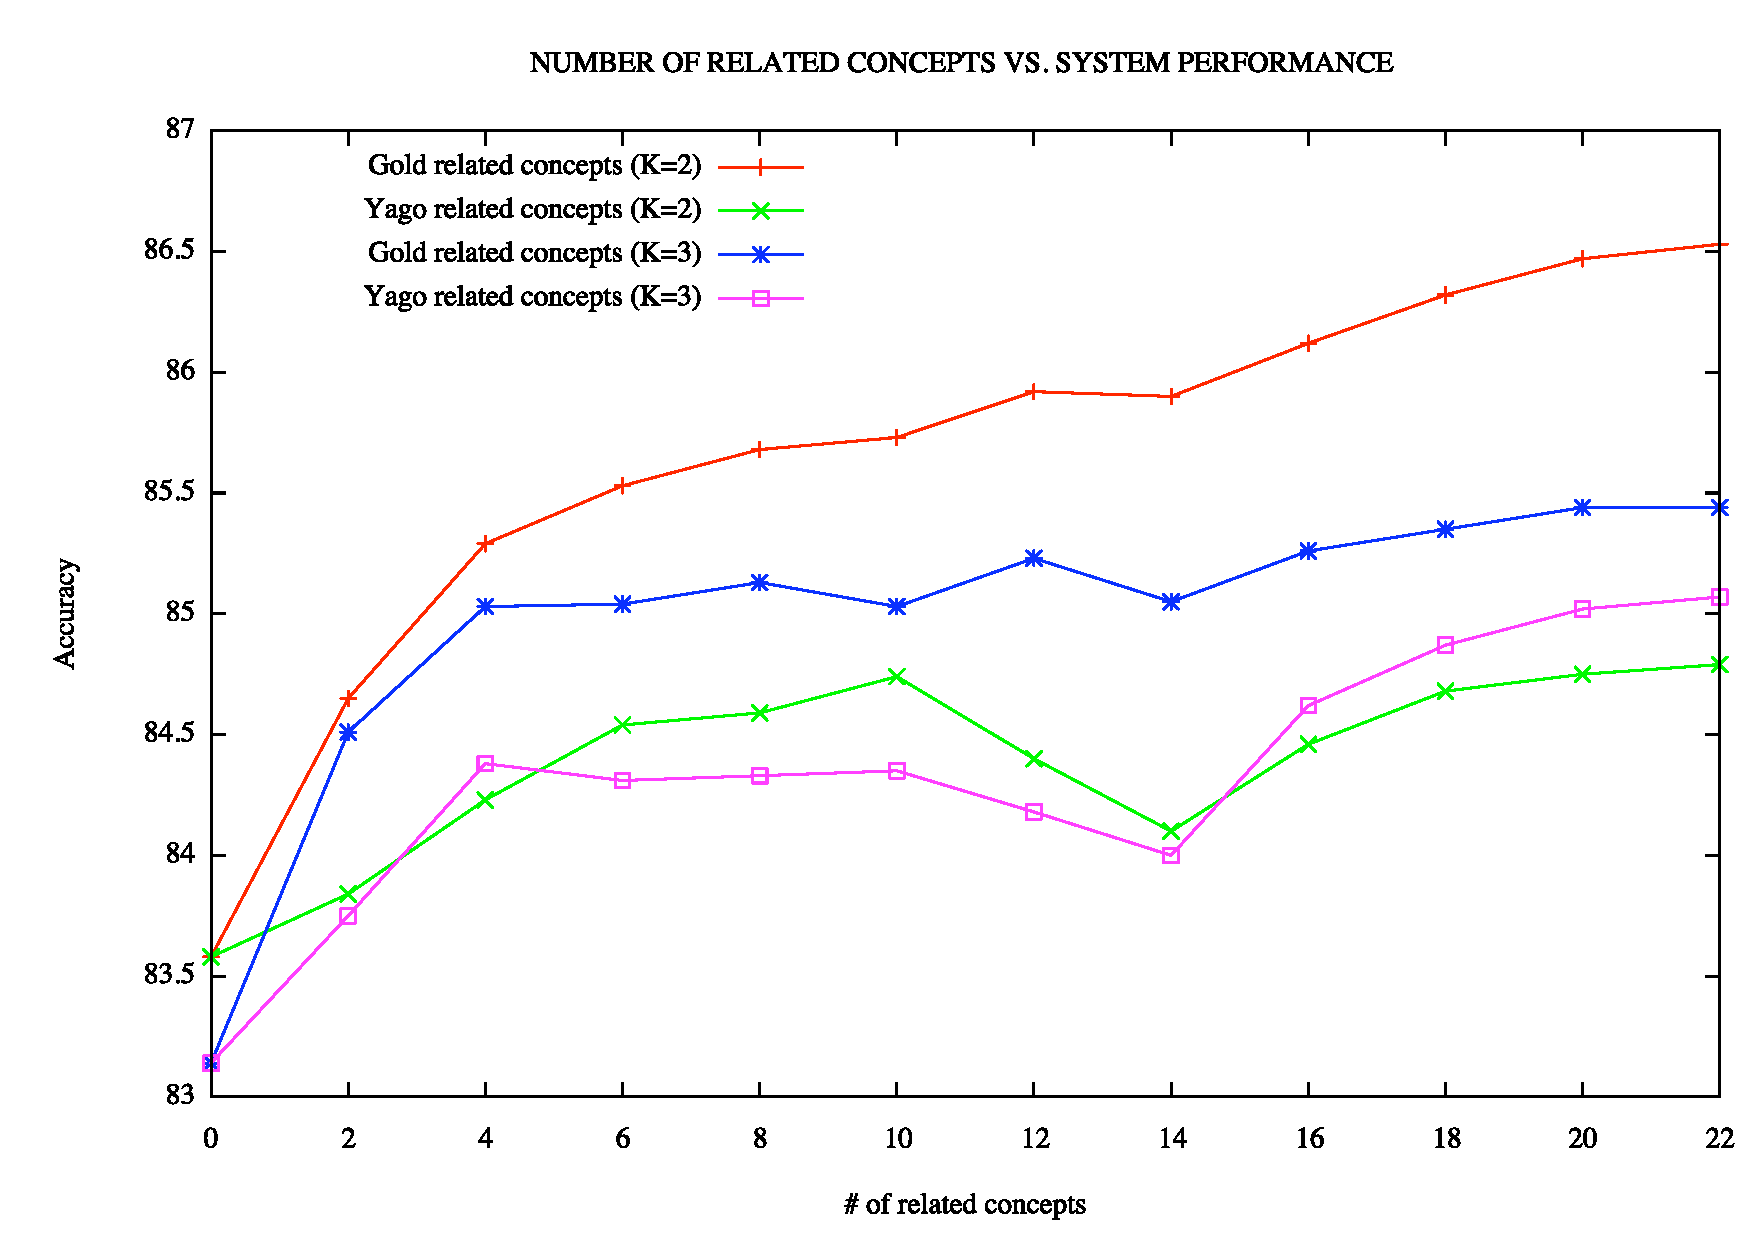
\includegraphics[totalheight=0.21\textheight]{relatedconcepts4}
  \caption{Relation between our system performance and the number of
    related concepts used in the constraint-based inference model.}
  \label{fig:related-concepts}
\end{figure}
}

\ignore{ In Sec. \ref{sec:rel-con-ext},  we propose the intuition that
  the more  relevant to the  input concepts the related  concepts are,
  the  better performance  the  system gets.  In  this experiment,  we
  empirically show the correctness  of the intuition by evaluating our
  best    system    with    inference    model   on    {\bf    Test-I}
  dataset.  Fig. \ref{fig:related-concepts} shows  the results  of the
  systems using  the inference  model with related  concepts extracted
  from the original dataset and from \textsc{Yago}.  }

%%%%%%%%%%%%%%%
% Old writing %
%%%%%%%%%%%%%%%

\ignore{Specifically, examples are created with the following
  guidelines.

  \begin{itemize}
  \item $X \leftarrow Y$ examples: For each semantic class, we pair
    the name of the class with its instances. These examples have the
    general form ({\em semantic class X}, {\em child of X}).
  \item $X \rightarrow Y$ examples: These examples have the general
    form ({\em concept X}, {\em semantic class of X}).
  \item $X \leftrightarrow Y$ examples: The general form of these
    examples is ({\em concept X}, {\em concept Y}), where $X$ and $Y$
    are two instances of a semantic class, and $X \ne Y$.
  \item $X \nleftrightarrow Y$ examples: To make examples with two
    concepts having no relation, we pair either a semantic class name
    and an instance of another semantic class (and vice versa), or an
    instance in a semantic class and another instance in other
    classes.
  \end{itemize}
}

\ignore{We refer to the 12,000-example test set as the {\em TestAll}
  test set. From the training set, we discard examples with one or
  both concepts not in Wikipedia ({\em non-Wikipedia examples}). This
  results in a training set of $6,959$ examples.  It is important to
  note that, we do not discard {\em non-Wikipedia} examples in the
  {\em TestAll} test set. Table \ref{tab:detail-dataset} shows the
  statistics of the training and test data.

  \begin{table}[!t]
    \small
    \begin{center}
      \begin{tabular}{|l||c|c|c|c|c|}
        \hline
        Data & $X \leftarrow Y$ & $X \rightarrow Y$  & $X \leftrightarrow Y$  & $X \nleftrightarrow Y$ & Total \\
        \hline
        \hline
        {\em Training}  & 1,739 & 1,754 & 1,664 & 1,802 & 6,959\\
        % {\em TestWiki} & 2,684 & 2,654 & 2,483 & 2,635 & 10,456 \\
        {\em TestAll} & 3,045 & 3,025 & 2,965 & 2,965 & 12,000 \\
        \hline
      \end{tabular}
      \caption{Details of the training and test sets with the number
        of examples in each relation class. The {\em Training} set
        contains only examples in Wikipedia. {\em TestAll} includes
        {\em non-Wikipedia} examples.}
      \label{tab:detail-dataset}
    \end{center}
  \end{table}
}

\ignore{Each semantic class is an incomplete set of representative
  instances and has about 272 instances in average. The smallest class
  is {\em search engine} with 25 instances, and the largest class is
  {\em actor} with 1500 instances. Table \ref{table:class-instance}
  shows a snippet of the dataset. We have both types of closed word
  semantic class (e.g. {\em chemical element}, {\em country}) and open
  word semantic class (e.g. {\em basic food}, {\em
    hurricane}). Moreover, there are classes with proper nouns
  (e.g. {\em actor} with {\em Mel Gibson}) and classes with common
  nouns (e.g. {\em basic food} with {\em rice}, {\em milk}).

  \begin{table}[!t]
    \small
    \centering
    \begin{tabular}{|r|l|}
      \hline
      \multicolumn{2}{|c|}{A snapshot of the original dataset} \\
      \hline
      \textbf{Semantic class (Size)} & \textbf{Examples of Instances} \\
      \hline
      \hline
      basic food (155) & rice, milk, eggs, beans, fish \\
      \hline
      chemical element (118) & lead, copper, aluminum, calcium \\
      \hline
      city (589) & San Francisco, Dubai, Chicago \\
      \hline
      disease (209) & arthritis, hypertension, influenza \\
      \hline
      actor (1500) & Kate Hudson, Mel Gibson \\
      \hline
    \end{tabular}
    \caption{A snippet of 40 semantic classes with instances. 
      The class names in the original dataset ({\em basicfood}, 
      {\em chemicalelem}) were presented in a meaningful form
      as shown in the left column.}
    \label{table:class-instance}
  \end{table}
}

\ignore{ Lucene is a high-performance text search library written in
  Java and widely used as an off-the-shelf IR system.}

\ignore{
  \begin{table}[!t]
    \small
    \begin{center}
      \begin{tabular}{|c||c|c|c|c|}
        \hline
        \multicolumn{5}{|c|}{Overall results and comparison} \\
        \hline
        $K$  &  \textsc{Strube 07}  &  \textsc{Snow 06}  &  \textsc{Yago 07}  &  \textsc{Ours}            \\
        \hline
        1  &      23.83  &    40.24  &           64.43  &  \textbf{82.13}  \\
        2  &      23.84  &    42.63  &           63.94  &  \textbf{84.79}  \\
        3  &      23.88  &    40.96  &           62.02  &  \textbf{85.07}  \\
        4  &      24.32  &    40.65  &           60.57  &  \textbf{84.08}  \\
        \hline
      \end{tabular}
      \caption{Performance of our overall system compared to other
        systems. Performances are measured by accuracy. The {\em
          TestAll} test set with $12,000$ examples is used in this
        experiment. $K$ is the number of levels to climb up in the
        hierarchical structure of knowledge sources as described in the
        text.}
      \label{table:compare-others}
    \end{center}
  \end{table}
}

\ignore{Our system also uses Wikipedia as its main background
  knowledge. However, ours is superior to other systems because it
  employs advance machine learning techniques along with a powerful
  and effective constraint-based inference model.}

\ignore{
  \begin{enumerate}

  \item \textsc{Strube 07} uses a large scale taxonomy which was
    derived from Wikipedia \cite{wikitaxo07}, as the background
    knowledge. The taxonomy was created by applying several lexical
    matching and methods based on connectivity in the network to the
    category system in Wikipedia. As a result, the taxonomy contains a
    large amount of subsumption, i.e. {\em isa}, relations
    \cite{wikitaxo07}. Given an input with two concepts $X$ and $Y$,
    using the taxonomy, $X$ is an ancestor of $Y$ if one of the
    articles about $Y$ is subsumed by an article about $Y$, using {\em
      isa} links of articles, up to $K$ levels in the taxonomy.
    Similarly, for the case that $Y$ is an ancestor of $X$. If $X$ and
    $Y$ share a common ancestor within $K$ levels in the taxonomy,
    they are considered siblings. We first apply our concept
    disambiguation algorithm on given concepts and then mount them
    onto the taxonomy to infer the relations. The taxonomy used in
    this experiment is in the latest version from March,
    2008\footnote{Private communication with Michael Strube and Simone
      Paolo Ponzetto, 2009.}.

  \item \textsc{Snow 06} uses the {\em augmented WordNet}
    \cite{ilprints665,Snow2006} as background knowledge. To build the
    {\em augmented WordNet}, the authors first identified
    lexico-syntactic patterns indicative of hypernymy from corpora and
    use them to extract candidate noun pairs that may hold the
    hypernym relation. A trained classifier is applied on these noun
    pairs to recognize the pairs holding hypernym relation. Starting
    from WordNet-2.1 \cite{Fellbaum98}, the latest version of the
    augmented WordNet has augmented 400,000 synsets. Words that are
    added into the augmented WordNet can be common nouns or proper
    nouns. The augmented WordNet can serve as effective background
    knowledge for identifying the relational knowledge of interest by
    looking for the input concepts in the augmented WordNet tree in all
    possible senses of the concepts and then inferring their
    relationship. We also vary the value of $K$ as the number of
    levels to go up on the WordNet tree from input concepts to find
    their common subsumptions.

  \item \textsc{Yago 07} uses YAGO ontology \cite{suchanek2007WWW} as
    the main source of background knowledge. Because YAGO ontology is
    a combination of Wikipedia and WordNet (see our brief description
    in Sec. \ref{sec:rel-con-ext}), this system is expected to be
    powerful in recognizing concept relationships. To access a
    concept's ancestors and siblings, we combine \textsc{Pattern 1} in
    Fig. \ref{alg:yago-query} and the \textsc{subClassOf} relation in
    YAGO model to go up on the ontology. The \textsc{subClassOf}
    relation can be cascaded $K$ times to climb up in the ontology.

  \end{enumerate}
}

\ignore{
Because the systems in the previous experiments do not use the same
source of background knowledge, we, furthermore, perform experiments
in which these systems are compared with different data sets covered
in different knowledge sources. This experiment provides a fair
comparison for systems that use different resources as their
background knowledge. New data sets are derived from the {\em TestAll}
test set. The first derived data set is {\em TestWiki} which contains
only {\em Wikipedia concepts}. By removing all examples with {\em
  non-Wikipedia concept}, there are $10,456$ examples remained in {\em
  TestWiki}. The second derived data set is {\em TestWn}, which
contains only concepts in the {\em augmented WordNet}
\cite{ilprints665,Snow2006}.  {\em TestWn} has $8,625$ examples after
dropping $3,375$ examples with concepts not in the {\em augmented
  WordNet} from {\em TestAll}.  The results of this experiment are
shown in Tab. \ref{table:exp-diff-test}.  We only report the best
results achieved by the systems on different test sets. Our system
still significantly outperforms other systems when compared on
specific data sets.

\begin{table}[!t]
  \small
  \begin{center}
    \begin{tabular}{|c||c|c|c|c|}
      \hline
      \multicolumn{5}{|c|}{Comparison on special data sets} \\
      \hline
      Data set &  \textsc{Strube 07}  &  \textsc{Snow 06}  &  \textsc{Yago 07}  &  \textsc{Ours}   \\
      \hline
      {\em TestWiki}  &               24.59  &             44.34  &             70.29  &  \textbf{90.92}  \\
      {\em TestWn}    &               24.13  &             47.79  &             70.81  &  \textbf{90.76}  \\
      \hline
    \end{tabular}
    \caption{Comparison of systems' performance with different test
      sets derived from the {\em TestAll} test set. {\em TestWiki}
      contains $10,456$ examples in Wikipedia, and {\em TestWn}
      contains $8,625$ examples in the {\em augmented WordNet}. The
      best performance of each system (by varying $K$) is reported.}
    \label{table:exp-diff-test}
  \end{center}
\end{table}
}

\ignore{
\begin{table*}[!t]
  \begin{center}
    \begin{tabular}{|l||c|c|c|}
      \hline
      \multicolumn{4}{|c|}{Constribution of the components in our system} \\
      \hline
      &         Results on $10,456$  &  Results on $1,544$              &         Overall results  \\
      System &  {\em Wikipedia examples}  &  {\em non-Wikipedia examples}  &  on $12,000$ examples  \\
      \hline
      \hline
      Baseline        &                       88.79  &                      31.22       &                   81.38  \\
      \hline
      w/o Inference   &                       88.79  &                      44.88       &                   83.14  \\
      \hline
      with Inference  &                       \textbf{90.92}  &                      \textbf{45.40}       &                   \textbf{85.07}  \\
      \hline
    \end{tabular}
    \caption{\small Contributions of the components in our system evaluated
      on three types of data. The first column shows results only on
      examples with concepts that appear in Wikipedia. The second
      column shows results on examples having concepts that do not
      appear in Wikipedia, and thus exhibits the power of our method
      to extend outside Wikipedia. The third column shows results on
      the overall data set, that consists of around 13\% of the
      concepts pairs that are outside Wikipedia. The {\em Baseline}
      system is our local relation classifier that uses neither the
      approach of finding replacements for {\em non-Wikipedia
        concepts} nor the inference model. The baseline on {\em
        non-Wikipedia examples} is computed by assuming sibling
      relation all the time. By adding the component of finding
      replacements for {\em non-Wikipedia concepts}, we have the {\em
        w/o Inference} system.}
    \label{tab:w-wo-infer}
  \end{center}
\end{table*}
}


\ignore{
  \subsubsection{Contributions of the Components in our System}

  In this experiment, we show the contribution of the components in
  our overall algorithm (see Fig. \ref{fig:rel-know-iden-alg}). We use
  different data sets in this experiments to study the variation in
  behavior of our system. The first data set is the {\em TestWiki} in
  the previous experiment. This test set contains $10,456$ examples
  with {\em Wikipedia concepts}. These are the remained examples after
  dropping {\em non-Wikipedia concepts} from $12,000$ examples in the
  {\em TestAll} test set. The second test set contain only $1,544$
  concept pairs with at least one {\em non-Wikipedia} concept in
  each. In other words, the second test set is the complement of the
  {\em TestWiki} test set with respect to the {\em TestAll} test
  set. The third test set is the {\em TestAll} test set. The results
  are shown in Tab. \ref{tab:w-wo-infer}.

  In Tab. \ref{tab:w-wo-infer}, the {\em Baseline} system is our local
  relation classifier that uses neither the component finding
  replacements for {\em non-Wikipedia concept} nor the
  constraint-based inference model. The baseline on {\em non-Wikipedia
    examples} is computed by assuming sibling relation all the
  time. In the {\em w/o Inference} row, we evaluate our system with
  the contribution of the component finding replacements for {\em
    non-Wikipedia concepts}, but inference model. The result on
  $10,456$ {\em Wikipedia examples} remains the same because, all of
  concepts in these examples are in Wikipedia, the system does not
  need to find replacement concepts. The significant improvement in
  the results on $1,544$ {\em non-Wikipedia examples} shows the
  effectiveness of our approach in finding replacements for {\em
    non-Wikipedia concepts}. Overall, we obtain almost $2\%$ of
  improvement in accuracy after adding the finding replacement
  component. The third experiment is carried out by evaluating our
  overall algorithm in Fig. \ref{fig:rel-know-iden-alg} on all test
  sets. The inference process significantly improve the results of our
  system on $10,456$ {\em Wikipedia examples}. It also gains
  improvements on the {\em non-Wikipedia examples} so that in overall,
  by adding the constraint-based inference component, the system
  improves $\sim 2\%$ in accuracy. Overall, our system achieves
  significant improvement reaching to $85.07\%$ accuracy in overall by
  adding in all components, compared to $81.38\%$ accuracy gained by
  the {\em Baseline} system.

  \begin{table*}[!t]
    \small
    \begin{center}
      \begin{tabular}{|c|c|c|c|c|c|c|c|}
        \hline
        No.  &  $X$             &  $Y$          &  True    &  LocalClassifier       &  \multicolumn{2}{|c|}{Replacement Needed?}  &  withInference \\ \cline{6-7}
        &                  &               &  Label   &  Prediction                   &  $X$                  &  $Y$                     &  Prediction           \\
        \hline
        \hline
        1&city                    &lisbon                   &$X \leftarrow Y$      &$X \leftarrow Y$      &(no)        &(no)         &$X \leftarrow Y$  \\
        2&{\em bartlomiej strobel}&painter                  &$X \rightarrow Y$     &$X \rightarrow Y$     &drew struzan&(no)         &$X \rightarrow Y$ \\
        3&taiwan                  &singapore                &$X \leftrightarrow Y$ &$X \leftarrow Y$               &(no)        &(no)         &$X \leftrightarrow Y$ \\
        4&jean ingres             &{\em harald slott-moller}&$X \leftrightarrow Y$ &$X \nleftrightarrow Y$         &(no)        &george inness&$X \leftrightarrow Y$ \\
        5&{\em southern herald}   &newspaper                &$X \rightarrow Y$     &$X \leftrightarrow Y$          &liberty     &(no)         &$X \rightarrow Y$  \\
        6&somalia                 &hurricane                &$X \nleftrightarrow Y$&$X \nleftrightarrow Y$&(no)        &(no)         &$X \leftrightarrow Y$  \\
        \hline
      \end{tabular}
      \caption{Relationship prediction examples from {\em TestAll}
        test set. Concepts in {\em italic font} are not in Wikipedia,
        and they are replaced by other {\em Wikipedia concepts} as
        shown.}
      \label{table:pre-examples}
    \end{center}
  \end{table*}
}

\ignore{
In our inference process, we used related concepts added to form
relational constraints in concept networks. The relational constraints
will then enforce concept networks to eliminate violated ones and pick
the best concept network available. From our inference model, we make
two following claims: (1) The more relevant to the input concepts the
related concepts are, the better performance the system gets, and (2)
the more related concepts added to the inference process, the better
performance the system gets.

To prove the first claim, we use the original data of forty semantic
classes (see Sec. \ref{sec:dataset}) to provide {\em gold related
  concepts} to the inference process as discussed in
Sec. \ref{sec:rel-con-ext}. Our experiment shows that by using this
approach, the performance of our best system reaches to $86.52\%$ in
accuracy on the {\em TestAll} test set, compared to $85.07\%$ accuracy
obtained when using another knowledge source to provide related
concepts. For the second claim, we evaluate our system with several
numbers of related concepts added to the inference process. In this
experiment, we use both the {\em gold related concepts} provided by
the original dataset and the {\em YAGO related concepts} extracted
from YAGO ontology (see Sec. \ref{sec:rel-con-ext}) for the inference
process.

Fig. \ref{fig:related-concepts} shows the improvement in the
performance of our system with respect to the quality of the related
concepts used and also the number of related concepts. This experiment
is done on the {\em TestAll} test set. It is shown clearly that the
related concepts from gold data outperform the related concepts
extract from the other source. Due to the quality of the related
concepts extracted from YAGO ontology, sometimes, adding more concepts
hurts the performance. We use $K=2$ and $K=3$ in this
experiment\footnote{$K$ is the number of levels to go up in the
  Wikipedia category system to extract features for input concept
  pairs.}. The related concepts include the ancestors, siblings, and
children of an input concept. For simplicity, in this experiment we
only report the total number of related concepts extracted for two
input concepts of an example.
}

\ignore{
  \subsubsection{System's Output Examples}

  Table \ref{table:pre-examples} shows some output examples of our
  overall system in Fig. \ref{fig:rel-know-iden-alg} (see column {\em
    withInference}). We also present the predictions made by the
  system without inference component ({\em LocalClassifier}). Concepts
  which are not in Wikipedia will be replaced by {\em Wikipedia
    concepts} ({\em Replacement Needed?}). Example \#1 and \#2 show
  two concept pairs correctly classified by both {\em LocalClassifier}
  and {\em with Inference}. Especially, in \#2, that concept {\em
    bartlomiej strobel} is replaced with {\em drew struzan} helps the
  systems make correct predictions. In examples \#3, {\em
    LocalClassifier} make incorrect predictions, but {\em
    withInference} remedies this. Example \#4 and \#5 show two cases
  where two {\em non-Wikipedia concepts} are correctly replaces with
  two corresponding {\em Wikipedia concepts}, but {\em
    LocalClassifier} still makes incorrect prediction. However, {\em
    withInference}, with its power of internal reasoning using
  relational constraints, proves to be successful. Example \#6 is an
  example where {\em LocalClassifier} makes correct prediction, but
  {\em withInference} does not. This is probably because of bad
  related concepts extracted for the two input concepts.  }


%%% Local Variables: 
%%% mode: latex
%%% TeX-master: "jupiter"
%%% End: 


\section{Discussion}
\label{sec:discussion}
%Discussion section. Open for anything to discuss about.

%- Discuss about the Sibling relation recognition alone: why it bad, why it good.
%- Discuss about the prominence doesn't work, move the algorithm to this section.

%- Perhaps, a analysis subsection in Experiment section to show the problem of sibling detector with different type of pair (classclass, entityentity, etc.)

%- Analysis on the detail accuracy of 40 classes

%- Answer the question: Is it correct that 

%While our ancestor relation identifier and our overall relation identification system significantly outperforms the baseline system, which uses the extended WordNet as the knowledge source, the precision of our cousin identifier needs to be improved. A detailed study shows that our cousin identifier tends to identify entity pairs as cousins. This can be explained by the noise in the Wikipedia data that make two irrelevant articles representing for two input entities may have common unexpected categories. Articles in Wikipedia are collaboratively created by many volunteers over the world. Therefore, maintaining a high quality of articles in the encyclopedia is not easy. This directly suggests a challenge of dealing with noise in this sort of knowledge source. We consider this as a challenge in our future work.

We experienced that the data set of 40 classes of instances we are using in this work mostly contains unambiguous entities (i.e., entities that do not share meanings with many other entities). We do not have ambiguous entities such as {\em Bush} or {\em Ford} in this dataset. Therefore, the prominence-based search (described in Section \ref{sec:prominence}) did not have a chance to display its ability of disambiguating entities. We evaluated our ancestor identifier without prominence-based search on the same test set we used in Experiment 1. We got 86.2\% in accuracy, compared to the accuracy of 86.4\% of the identifier with prominence-based search. However, we manually selected a list of several commonly used name entities such as {\em Bush}, {\em Ford}, {\em Gates}, {\em Jobs}, etc., and tried our search engine on this list. We got the important people that we want to know about most of the time. This implies that our system potentially works well on other data sets which may contain ambiguous entities.


\section{Conclusion}
\label{sec:conclusion}
We studied an important component of many computational linguistics
tasks -- identifying taxonomic relations between pairs of concepts. We
argued and provided experimental evidences that static structured
knowledge bases cannot support this task well enough. We developed
TREI, a novel algorithm that leverages information from existing
knowledge sources and uses machine learning and a constraint-based
inference model to get around the noise and the level of uncertainty
inherent in these resources. The experimental study showed that TREI
is significantly better than other systems which were built upon
existing well-known structured resources. Our approach generalized
well across semantic classes and handled well non-Wikipedia
concepts. Our future research will include an evaluation of TREI in
the context of textual inference applications.

\ignore{The key lesson from the success of our approach has to do with
  our combined learning and global inference approach. Furthermore, we
  demonstrate an effective approach to leveraging existing knowledge
  bases for this inference process.}

\ignore{Our machine learning approach makes use of Wikipedia resource,
  but views it as an open and noisy resource; this is augmented with a
  novel use of a constraint-based inference model that allows us to
  make these decisions more robust.}  \ignore{The key technical step
  needed to improve our method further is to better generate concepts
  that are related to the target concepts, so that our global
  inference method becomes even more effective.}

%%% Local Variables:
%%% mode: latex
%%% TeX-master: "jupiter"
%%% End:



\bibliographystyle{acl}
\bibliography{jupiter,ccg,cited}

\end{document}

%%% Local Variables: 
%%% mode: latex
%%% TeX-master:
%%% End: 
